
\documentclass{article}
\usepackage{amstext,amssymb,amsmath,amsbsy}
\usepackage[utf8]{inputenc}

\usepackage{graphicx}
\usepackage{subfigure}
\usepackage{calc}
\usepackage{color}
\usepackage{float}

\newcommand{\Db}[1]{\Delta\bar{#1}}
\newcommand{\E}{\mathbb{E}}
\newcommand{\Ep}[1]{\mathbb{E} \left( #1 \right)}
\newcommand{\In}{\text{In}}
\newcommand{\Iniv}{\text{In}_\text{iv}(t)}
\newcommand{\Insc}{\text{In}_\text{sc}(t)}
\newcommand{\tss}{t_\text{ss}}
\newcommand{\Ccrit}{C_\text{crit}}
\newcommand{\Cnonlin}{C_\text{crit}}
\newcommand{\CAFIR}{C^*_\text{AFIR}}
\newcommand{\dd}{\text{d}}
\newcommand{\e}{\text{e}}
\newcommand{\syn}{\text{syn}}
\newcommand{\tot}{\text{tot}}
\newcommand{\acc}{\text{acc}}
\newcommand{\avg}{\text{avg}}
\newcommand{\kat}{k_\text{aT}}
\newcommand{\Tin}{T_\text{in}}
\newcommand{\on}{\text{on}}
\newcommand{\off}{\text{off}}
\newcommand{\kon}{k_{\text{on}}}
\newcommand{\koff}{k_{\text{off}}}
\newcommand{\keD}{k_\text{eD}}
\newcommand{\keR}{k_\text{eR}}
\newcommand{\keT}{k_\text{eT}}
\newcommand{\keDT}{k_\text{eDT}}
\newcommand{\keC}{k_\text{eC}}
\newcommand{\keCR}{k_\text{eCR}}
\newcommand{\kcp}{k_{12}}
\newcommand{\kpc}{k_{21}}
\newcommand{\ka}{k_\text{a}}
\newcommand{\ke}{k_\text{e}}
\newcommand{\Vc}{V_\text{c}}
\newcommand{\Vp}{V_\text{p}}
\newcommand{\Vm}{V_\text{m}}
\newcommand{\Vmax}{V_\text{max}}
\newcommand{\Km}{K_\text{m}}
\newcommand{\Kd}{K_\text{d}}
\newcommand{\Kss}{K_\text{ss}}
\newcommand{\Keq}{K_\text{eq}}
\newcommand{\Keqp}{K_\text{eqp}}
\newcommand{\KeqM}{K_\text{eqM}}
\newcommand{\KD}{K_\text{DT}}
\newcommand{\KN}{K_\text{TN}}
\newcommand{\ksyn}{k_{\text{syn}}}
\newcommand{\ksynp}{k_{\text{synp}}}
\newcommand{\ksynM}{k_{\text{synM}}}
\newcommand{\kint}{k_{\text{int}}}
\newcommand{\kdeg}{k_{\text{deg}}}
\newcommand{\Cdep}{C_\text{dep}}
\newcommand{\Ddep}{D_\text{dep}}
\newcommand{\Ctot}{C_\text{tot}}
\newcommand{\Rtot}{R_\text{tot}}
\newcommand{\Dtot}{D_\text{tot}}
\newcommand{\Ttot}{T_\text{tot}}
\newcommand{\Ntot}{N_\text{tot}}
\newcommand{\DT}{\textit{DT}}
\newcommand{\Dtotinit}{D_{\text{tot0}}}
\newcommand{\Ttotinit}{T_{\text{tot0}}}
\newcommand{\Rtotinit}{R_{\text{tot0}}}
\newcommand{\Cavg}{C_\text{avg}}
\newcommand{\Cavgss}{C_\text{avg,ss}}
\newcommand{\Dtotmax}{D_\text{tot,max}}
\newcommand{\Dtotavg}{D_\text{tot,avg}}
\newcommand{\Dtotmin}{D_\text{tot,min}}
\newcommand{\Ttotavg}{T_\text{tot,avg}}
\newcommand{\Ttotmax}{T_\text{tot,max}}
\newcommand{\Ttotmin}{T_\text{tot,min}}
\newcommand{\Dcorr}{D_{\text{corr0}}}
\newcommand{\Dss}{D_\text{ss}}
\newcommand{\Tss}{T_\text{ss}}
\newcommand{\Tavg}{T_\text{avg}}
\newcommand{\Tmax}{T_\text{max}}
\newcommand{\Tavgqe}{T_\text{avg}^\text{QE}}
\newcommand{\Tmaxqe}{T_\text{max}^\text{QE}}
\newcommand{\Dtotss}{D_\text{tot,ss}}
\newcommand{\Ttotss}{T_\text{tot,ss}}
\newcommand{\Ctotss}{C_\text{tot,ss}}
\newcommand{\Rtotss}{R_\text{tot,ss}}
\newcommand{\Dmin}{D_\text{min}}
\newcommand{\Emax}{E_\text{max}}
\newcommand{\Cmin}{C_\text{min}}
\newcommand{\tmax}{t_\text{max}}
\newcommand{\Acc}{\text{Acc}}
\newcommand{\Tacc}{T_\text{acc}}
\newcommand{\Nacc}{N_\text{acc}}
\newcommand{\Racc}{R_\text{acc}}
\newcommand{\Accavg}{\text{Acc}_\text{avg}}
\newcommand{\Accmax}{\text{Acc}_\text{max}}
\newcommand{\Accmin}{\text{Acc}_\text{min}}
\newcommand{\wt}{\text{WT}}
\newcommand{\Dose}{\text{Dose}}
\newcommand{\CL}{CL}
\newcommand{\CLtm}{CL_{TM}}
\newcommand{\CLtmmax}{CL_{TM,max}}
\newcommand{\Cafir}{C_\text{AFIR}}
\newcommand{\Cafirss}{C_\text{AFIRss}}
\newcommand{\SCR}{\text{SCR}}
\newcommand{\ASCR}{\text{ASCR}}
\newcommand{\AFIR}{\text{AFIR}}
\newcommand{\TFIR}{\text{TFIR}}
\newcommand{\AFIRT}{\text{AFIRT}}
\newcommand{\PFI}{\text{PFI}}
\newcommand{\AFIRavg}{\text{AFIR}_\text{avg}}
\newcommand{\TFIRavg}{\text{TFIR}_\text{avg}}
\newcommand{\AFIRqe}{\text{AFIR}_\text{QE}}
\newcommand{\TFIRqe}{\text{TFIR}_\text{QE}}
\newcommand{\AFIRdet}{\text{AFIR}\vert_{\Dtot \sim \Ttot}}
\newcommand{\TFIRdet}{\text{TFIR}\vert_{\Dtot \sim \Ttot}}
\newcommand{\AFIRib}{\text{AFIR}_\text{IB}}
\newcommand{\TFIRib}{\text{TFIR}_\text{IB}}
\newcommand{\MW}{\text{MW}}
\newcommand{\LOQ}{\text{LOQ}}

\newcommand{\tis}{\textrm{tis}}
\newcommand{\pla}{\textrm{pla}}
\newcommand{\Ctis}{C_\textrm{tis}}
\newcommand{\CLtis}{\textrm{CL}_\textrm{int,tis}}
\newcommand{\Vtis}{V_\textrm{tis}}
\newcommand{\Ktis}{K_\textrm{tis}}
\newcommand{\Khat}{\hat{K}_\textrm{tis}}
\newcommand{\Rtis}{R_\textrm{tis}}
\newcommand{\Etis}{E_\textrm{tis}}
\newcommand{\Ltis}{L_\textrm{tis}}
\newcommand{\stis}{\sigma_\textrm{tis}}
\newcommand{\ABCtis}{\textrm{ABC}_\textrm{tis}}
\newcommand{\ABCexp}{\textrm{ABC}_\textrm{exp}}
\newcommand{\ABC}{\text{ABC}}
\newcommand{\Cpla}{C_\textrm{pla}}
\newcommand{\Vpla}{V_\textrm{pla}}
\newcommand{\Khatpla}{\hat{K}_\textrm{pla}}
\newcommand{\spla}{\sigma_\textrm{pla}}

\newcommand{\subsubsubsection}[1]{\paragraph{#1}\mbox{}\\}



\renewcommand{\vector}[2]{
\left[\begin{array}{c}
    {#1} \\
    {#2}
    \end{array}\right]
}
\renewcommand{\matrix}[4]{
\left[\begin{array}{cc}
    {#1} & {#2} \\
    {#3} & {#4}
    \end{array}\right]
}

\date{}

\begin{document}
{\Large{\bf AFIRT: A Dimensionless Potency Metric for Characterizing the Activity of Monoclonal Antibodies in Target Tissue}} 
~
\\
\\
Abstract Word Count: XYZ
\\
Body Word Count (including figure captions): XYZ
\\
Number of Figures: XYZ 
\\
Number of Tables: XYZ
\\
Keywords: monoclonal antibody $|$ target mediated drug disposition $|$ pharmacokinetics and pharmacodynamics $|$ pharmacometrics

\bigskip

\def\thefootnote{\arabic{footnote}}
\begin{center}
    Andrew M. Stein\footnote{Novartis Institute for BioMedical Research, 45 Sidney St, Cambridge MA, 02140 USA, andrew.stein@novartis.com},
    Sameed Ahmed\footnote{Departments of Mathematics, University of South Carolina, ahmed3@math.sc.edu},
    Miandra Ellis\footnote{School of Mathematical and Statistical Sciences, Arizona State University, mellis5@asu.edu},
    Ngartelbaye Guerngar\footnote{Department of Mathematics and Statistics, Auburn University, nzg0017@auburn.edu},
    Hongshan Li\footnote{Department of Mathematics, Purdue University, li108@purdue.edu},
    Luca Pallucchini\footnote{Department of Mathematics, Temple University,  luca.pallucchini@temple.edu}
\end{center}

\tableofcontents

Figure are in a separate file at the end of this document.  They'll images themselves will need to be removed for CPT:PSP (06-Figures.tex). 

\section*{Abstract}
XYZ
\\
\\

\newpage
\section{Introduction}
In the development of biologics, understanding target engagement at the site of action plays a critical role in dose regimen selection \cite{wang16}.  As measurements at the site of action are often impossible to obtain, model based predictions of target engagement are often used to help justify the dose selection.  For example, for the PD-1 inhibitor pembrolizumab, a physiologically based model for antibody distribution and target engagement was developed to predict the dose needed to achieve target engagement and tumor suppression \cite{lindauer17}.  For the PD-L1 inhibitor atezolizumab, a much simpler approach was taken to help justify the dose regimen, where a particular tumor biodistribution coefficient ($B$) and in vivo binding affinity ($\Kd$) was assumed, the steady state trough concentration ($\Cmin$) was estimated from clinical observation and then the receptor occupancy ($RO$) formula in Equation~\ref{eq:ro} was used to identify the dosing regimen that would provide the drug concentration needed to achieve 95\% target occupancy.
\begin{equation}
RO = B\cdot\Cmin/(B\cdot\Cmin+\Kd)
\label{eq:ro}
\end{equation}

The advantage of using the complex, mechanistic model as done for pembrolizumab is that ideally, it captures all essential underlying physiology processes in making the dose regimen prediction.  The disadvantage of this approach however is that physiological models can be complex, making them difficult time consuming to develop and difficult to explain to collaborators.  The advantage using the simple RO formula as done for atezolizumab is that it is fast, easy to implement, and easy to explain to collaborators.  The disadvantage, however, is that it is not obvious that Equation~\ref{eq:ro} is appropriate to the clinical scenario as this equation was derived for the in vitro setting \cite{boeynaems80} where the was no drug distribution, target distribution, receptor synthesis, or receptor turnover.

In this paper, an analysis of the target mediated drug distribution system is is performed with the goal of deriving a simple expression for target engagement in the clinical scenario.  This work provides a simple expression for target engagement in the tissue of interest, extending previous work characterizing the Average Free target to Initial target Ratio (AFIR) at steady state in circulation \cite{stein17}.
\section*{Theory}

The drug and target dynamics are modeled with the following system of ordinary differential equations.  The model is shown in Figure~\ref{fig:model}.  THOUGH THIS FIGURE PROBABLY NEEDS TO BE UPDATED.
\begin{align}
\frac{dD_1}{dt} &= \frac{1}{V_C}\text{Dose}_{iv}(t) - k_{12D}D_1 + \frac{V_{D_2}}{V_{D_1}}k_{21D}D_2 - k_{13D}D_1 \nonumber 
+ \frac{V_{D_3}}{V_{D_1}}k_{31D}D_3\\& - k_{eD1}D_1 - k_{\text{on}1}D_1 \cdot S_1 + k_{\text{off}1}(DS_1)- k_{\text{on}1}D_1 \cdot M_1 + k_{\text{off}1}(DM_1)  \\
\frac{dD_2}{dt} &= k_{12D}\frac{V_{D_1}}{V_{D_2}}D_1 - k_{21D}D_2 \\
\frac{dD_3}{dt} &= \frac{V_{D_1}}{V_{D_3}}k_{13D}D_1 - k_{31D}D_3 - k_{eD3}D_3- k_{\text{on}3}D_3 \cdot M_3 + k_{\text{off}3}(DM_3)\nonumber  \\&- k_{\text{on}3}D_3 \cdot S_3 + k_{\text{off}3}(DS_3) \\
\frac{dM_1}{dt} &= k_{\text{syn}M1}-k_{\text{shed}M_1}M_1 - k_{13M}M_1 + \frac{V_{M_3}}{V_{M_1}}k_{31M}M_3- k_{eM1}M_1\nonumber  \\&- k_{\text{on}1}D_1 \cdot M_1 + k_{\text{off}1}(DM_1)  \\
\frac{dM_3}{dt} &= k_{\text{syn}3}-k_{\text{shed}M_3}M_3  + \frac{V_{M_1}}{V_{M_3}}k_{13M}M_1 - k_{31M}M_3 - k_{eM3}M_3-\nonumber \\& k_{\text{on}3}D_3 \cdot M_3 + k_{\text{off}3}(DM_3) \\
\frac{dS_1}{dt} &= k_{\text{syn}S1}+k_{\text{shed}M_1}M_1  - k_{13S}S_1 + \frac{V_{S_3}}{V_{S_1}}k_{31S}S_3 - k_{eS1}S_1 - k_{\text{on}1}D_1 \cdot S_1 \nonumber\\ & + k_{\text{off}1}(DS_1)  \\
\frac{dS_3}{dt} &= k_{\text{syn}S3}+k_{\text{shed}M_3}M_3  - k_{31S}S_3 + \frac{V_{S_1}}{V_{S_3}}k_{13S}S_1 - k_{eS3}S_3 - k_{\text{on}3}D_3 \cdot S_3 \nonumber\\ & + k_{\text{off}3}(DS_3)  \\
\frac{d(DM_1)}{dt} &=-k_{\text{shed}DM_1}DM_1 - k_{13DM}(DM_1) + \frac{V_{DM_3}}{V_{DM_1}}k_{31DM}(DM_3)  - k_{eDM1}DM_1\nonumber\\&+k_{\text{on}1}D_1 \cdot M_1 - k_{\text{off}1}(DM_1)  \\
\frac{d(DM_3)}{dt} &= -k_{\text{shed}DM_3}DM_3 - k_{31DM}(DM_3) + \frac{V_{DM_1}}{V_{DM_3}}k_{13DM}(DM_1)  - k_{eDM3}DM_3\nonumber \\&+k_{\text{on}3}D_3 \cdot M_3 - k_{\text{off}3}(DM_3)  \\
\frac{d(DS_1)}{dt} &=-k_{\text{shed}DM_3}DS_1  - k_{13DS}DS_1 + \frac{V_{DS_3}}{V_{DS_1}}k_{31DS}DS_3 - k_{eDS1}(DS_1)  \nonumber\\ &+ k_{\text{on}1}D_1 \cdot S_1 - k_{\text{off}1}(DS_1)  \\
\frac{d(DS_3)}{dt} &=-k_{\text{shed}DM_3}DS_3  - k_{31DS}DS_3 + \frac{V_{DS_1}}{V_{DS_3}}k_{13DS}DS_1 - k_{eDS3}(DS_3)  \nonumber\\ &+ k_{\text{on}3}D_1 \cdot S_3 - k_{\text{off}1}(DS_3)  
\end{align}

This model is considering three compartments like Model C but it is taking into account the possibility for the target to shad, i.e. the target in the previous models is always membrane-bound but in reality it can shad into the blood and into the tumor. We are also adding the lymphocyte trafficking ($k_{13M}$ and $k_{31M}$).
The analysis we are carrying out on this model is similar to the one done for model C with the required modification. For the first time we are calculating the AFIRT using an alternative approximations to the quasi-equilibrium (QE), the quasi-steady state (QSS) and the quasi-steady state xxxxxxx (QSSD). The quasi-steady state approximation assumed that $-k_{\text{shed}DM_3}DM_3 - k_{eDM3}DM_3+k_{\text{on}3}D_3 \cdot M_3 - k_{\text{off}3}(DM_3) = 0 $, similarly as before for $k_d$ we define $k_{ss}=\frac{k_{\text{shed}DM_3} + k_{eDM3}+ k_{\text{off}3}}{k_{\text{on}3}}$. 
The quasi-steady state xxxxxxx approximation assumed that $-k_{\text{shed}DM_3}DM_3-k_{31DM}(DM_3) - k_{eDM3}DM_3+k_{\text{on}3}D_3 \cdot M_3 - k_{\text{off}3}(DM_3) = 0 $, we define $k_{ssd}=\frac{k_{\text{shed}DM_3} +k_{31DM}+ k_{eDM3}+ k_{\text{off}3}}{k_{\text{on}3}}$. 
These approximations are obtained from equation (16) at steady state, i.e. $\frac{d(DM_3)}{dt}=0$, and assuming the terms $ \frac{V_{DM_1}}{V_{DM_3}}k_{13DM}(DM_1)$ and $ k_{31DM}(DM_3) $ are negligible for the QSS. We assume that only $\frac{V_{DM_1}}{V_{DM_3}}k_{13DM}(DM_1)$ is negligible for the QSSD. 

We obtain the following approximations 
\begin{align*}
\text{AFIRT} \approx k_{ssd}\frac{M_{3\text{tot,ss}}}{M_{3,0}}\frac{\text{CL}\times\tau}{\text{B}\times\text{Dose}},\\
\text{AFIRT} \approx k_{ss}\frac{M_{3\text{tot,ss}}}{M_{3,0}}\frac{\text{CL}\times\tau}{\text{B}\times\text{Dose}},\\
\text{AFIRT} \approx k_{d}\frac{M_{3\text{tot,ss}}}{M_{3,0}}\frac{\text{CL}\times\tau}{\text{B}\times\text{Dose}},
\end{align*}  
where 
\begin{align*}
M_{3\text{tot,ss}}&=\frac{k_{13DM}(V_C/V_T)k_{\text{syn}M1}+(k_{eDM1}+k_{\text{shed}DM_1}+k_{13DM})k_{\text{syn}M3}}{(k_{eDM1}+k_{\text{shed}DM_1}+k_{13DM})(k_{eDM3}+k_{\text{shed}DM_3}+k_{31DM})-k_{31DM}k_{13DM}},\\
M_{3,0}&=\frac{k_{13M}(V_C/V_T)k_{\text{syn}M1}+(k_{eM1}+k_{\text{shed}M_1}+k_{13M})k_{\text{syn}M3}}{(k_{eM1}+k_{\text{shed}M_1}+k_{13M})(k_{eM3}+k_{\text{shed}M_3}+k_{31M})-k_{31M}k_{13M}},\\
\text{B}&=\frac{k_{13D}(V_C/V_T)}{k_{eD3}+k_{31D}}.
\end{align*}
We can notice from the picture below that the approximation obtained using the (QSS) hypothesis gives better results than the one using (QE).

% ---------------------------------------------------------------
% Soluble Target 
% ---------------------------------------------------------------
\section{Soluble target at Initial State and Steady State}
\subsection{Some formulas}
With the same notations as in the sections above.\newline 
\textbf{At initial state}, we have
\begin{align*}
    \frac{dS_1}{dt} & = 0 \\
    \frac{dS_3}{dt} & = 0 \\
                M_1 & = M_{10} \\
                M_3 & = M_{30} \\
                D_1 & = 0 \\
                D_3 & = 0 \\
               DS_1 & = 0 \\
               DS_3 & = 0 
\end{align*}
So ODE 13 and 14 give us the following linear system
\[
    \matrix{-(k_{13S} + k_{eS1})}{\frac{V_T}{V_C}k_{31S}}{\frac{V_C}{V_T}k_{13S}}{-(k_{31S} + k_{eS3})}
        \cdot \vector{S_1}{S_3}_0 = \vector{-k_{synS1} - k_{shedM1}M_{10}}{-k_{synS3} - k_{shedM3}M_{30}}.
\]
So the initial soluble target concentration in the central and tumor compartment is
\begin{align}
    S_{10} & = \frac{(k_{31S} + k_{eS3})\cdot(k_{synS1} + k_{shedM1}M_{10})
                    + \frac{V_T}{V_C}k_{31S}(k_{synS3} + k_{shedM3}M_{30})}
                {(k_{13S} + k_{eS1})(k_{31S} + k_{eS3}) - k_{13S}k_{31S}} \\
    S_{30} & = \frac{\frac{V_C}{V_T}\cdot k_{13S}\cdot(k_{synS1} + k_{shedM1}M_{10})
                    + (k_{13S} + k_{eS1})(k_{synS3} + k_{shedM3}M_{30})}
            {(k_{13S} + k_{eS1})(k_{31S} + k_{eS3}) - k_{13S}k_{31S}}.
\end{align}

\textbf{At steady state}, we assume that all soluble target are in the form of bounded complex.
By the symmetry of our model, we have
\begin{align*}
    S_{1tot,ss} & = \frac{(k_{31DS} + k_{eDS3})\cdot(k_{synS1} + k_{shedDM1}M_{1tot,ss})
                    + \frac{V_T}{V_C}k_{31DS}(k_{synS3} + k_{shedDM3}M_{3tot,ss})}
                {(k_{13DS} + k_{eDS1})(k_{31DS} + k_{eDS3}) - k_{13DS}k_{31DS}} \\
    S_{3tot,ss} & = \frac{\frac{V_C}{V_T} k_{13DS}\cdot(k_{synS1} + k_{shedDM1}M_{1tot,ss})
                    + (k_{13DS} + k_{eDS1})(k_{synS3} + k_{shedDM3}M_{3tot3,ss})}
            {(k_{13DS} + k_{eDS1})(k_{31DS} + k_{eDS3}) - k_{13DS}k_{31DS}}
\end{align*}

Formulas for computing membrane target at initial and steady state can be found in 
\emph{Model F Appendix}, for convenience, we include them below

\newcommand{\Det}{(k_{shedM1} + k_{13M} + k_{eM1})(k_{shedM3} + k_{31M} + k_{eM3}) - k_{13M}k_{31M}}

\newcommand{\DetSS}{(k_{shedDM1} + k_{13DM} + k_{eDM1})(k_{shedDM3} + k_{31DM} + k_{eDM3})
- k_{13DM}k_{31DM}}
\begin{align*}
    M_{10} & = \frac{(k_{shedM3} + k_{31M} + k_{eM3})k_{synM1} + \frac{V_T}{V_C}k_{31M}k_{synM3}}
                    {\Det} \\
    M_{30} & = \frac{\frac{V_C}{V_T}k_{13M}k_{synM1} + (k_{shedM1} + k_{13M} + k_{eM1})k_{synM1}}
                    {\Det} \\
    M_{1tot,ss} & = \frac{(k_{shedDM3} + k_{31DM} + k_{eDM3})k_{synM1} + 
                            \frac{V_T}{V_C}k_{31DM}k_{synM3}}
                    {\DetSS} \\
    M_{3tot,ss} & = \frac{\frac{V_C}{V_T}k_{13DM}k_{synM1} + 
                            (k_{shedDM1} + k_{13DM} + k_{eDM1})k_{synM1}}
                    {\DetSS}
\end{align*}


\subsection{Pseudo-Code for extending the core functions}
The formulas to compute various AFIRTS for soluble targets in the tumor compartment are 
\begin{align}
    \text{AFIRTS.Kssd} & = \text{Kssd.S}\times \frac{\text{Tacc.tum.S}}{\text{B}\times C_{avg1}} \\
    \text{AFIRTS.Kss}  & = \text{Kss.S}\times \frac{\text{Tacc.tum.S}}{\text{B}\times C_{avg1}} \\
    \text{AFIRTS.Kd}   & = \text{Kd.S}\times \frac{\text{Tacc.tum.S}}{\text{B}\times C_{avg1}} \\
\end{align}
Where $\text{Kssd.S}$, $\text{Kss.S}$ and $\text{Kd.S}$
\begin{align}
    \text{Kssd.S} & = \frac{k_{shedDM3} + k_{31DS} + k_{eDS} + k_{off3}}{k_{on3}} \\
    \text{Kss.S}  & = \frac{k_{shedDM3} + k_{eDS} + k_{off3}}{k_{on3}} \\
    \text{Kd.S}   & = \frac{k_{off3}}{k_{on3}} \\
\end{align}
 Finally,
\begin{align}
    \text{Tacc.tum.S} = \text{S3tot.ss} / \text{S30}
\end{align}


To compute AFIRT for soluable target from simulation, do
\begin{enumerate}
\item compute $\text{Sfree.pct}:=\frac{S_3}{S_{30}}$
\item take the average of Sfree.pct in the steady steady state
\item return the result from step 2
\end{enumerate}



% ---------------------------------------------------------------
% Similarity Transform
% ---------------------------------------------------------------

\section{Similarity Transform}

We consider the model in Figure 1. A drug $(D)$ binds to its target $(M)$ to form a complex $(DM)$. It has three compartments, central, tissue, and peripheral.

The drug and target dynamics are modeled with the following system of ordinary differential equations
\begin{align}
\frac{dD_1}{dt} &= \frac{1}{V_1}\text{Dose}_{iv}(t) - k_{12D}D_1 + \frac{V_3}{V_1}k_{21D}D_2 - k_{13D}D_1 \nonumber \\
&+ \frac{V_2}{V_1}k_{31D}D_3 - k_{\text{on}1}D_1 \cdot M_1 + k_{\text{off}1}(DM_1) - k_{eD1}D_1 \\
\frac{dD_2}{dt} &= k_{12D}\frac{V_1}{V_3}D_1 - k_{21D}D_2 \\
\frac{dD_3}{dt} &= \frac{V_1}{V_2}k_{13D}D_1 - k_{31D}D_3 - k_{\text{on}3}D_3 \cdot M_3 + k_{\text{off}3}(DM_3) - k_{eD3}D_3 \\
\frac{dM_1}{dt} &= k_{\text{syn}1} - k_{13M}M_1 + \frac{V_2}{V_1}k_{31M}M_3 - k_{\text{on}1}D_1 \cdot M_1 + k_{\text{off}1}(DM_1) \nonumber \\ 
&- k_{eM1}M_1 \\
\frac{dM_3}{dt} &= k_{\text{syn}3} + \frac{V_1}{V_2}k_{13M}M_1 - k_{31M}M_3 - k_{\text{on}3}D_3 \cdot M_3 + k_{\text{off}3}(DM_3) \nonumber \\ 
&- k_{eM3}M_3 \\
\frac{d(DM_1)}{dt} &= - k_{13DM}(DM_1) + \frac{V_2}{V_1}k_{31DM}(DM_3) + k_{\text{on}1}D_1 \cdot M_1 - k_{\text{off}1}(DM_1) \nonumber \\ 
&- k_{eDM1}(DM_1) \\
\frac{d(DM_3)}{dt} &= \frac{V_1}{V_2}k_{13DM}(DM_1) - k_{31DM}(DM_3) + k_{\text{on}3}D_3 \cdot M_3 - k_{\text{off}3}(DM_3) \nonumber \\ 
&- k_{eDM3}(DM_3) \\
\end{align}

We will calculate $D_{\text{tot,avg}3}$, which is the average drug concentration at steady state in the tissue. We have $D_{\text{tot,avg}3} = B \cdot D_{\text{tot,avg}1}$, where $D_{\text{tot,avg}1}$ is the average drug concentration at steady state in the central, and $B$ is the antibody biodistribution coefficient. Assume that drug elimination only occurs in the central compartment, i.e., $k_{eD3} = 0$. Then for drugs dosed with linear PK at regular intervals and concentration much larger than target concentration, we have $D_{\text{tot,avg}1} = \text{Dose}/(CL \cdot \tau)$, where $CL = k_{eD1} \cdot V_1$ is the drug clearance [CITE REFERENCE 25 FROM AFIR ARTICLE]. \\

For the model with drug elimination in both the central and tissue compartments, we will derive an alternative model with $k_{eD3} = 0$ that is indistinguishable from the existing model by using the similarity transform technique [CITE GODFREY 1989]. We consider drug concentration large enough that target binding does not affect drug distribution. Then the model equations for the drug can be written as 
\begin{align}
\frac{d\mathbf{D}}{dt} = A \cdot \mathbf{D}(t) + B \cdot Dose_{iv}(t), \label{model matrix}
\end{align}
with measurement
\begin{align}
\mathbf{m}(t) = C \cdot \mathbf{D}(t), \label{measurement matrix}
\end{align}
where
\begin{align}
\mathbf{D} = \begin{pmatrix}
D_1 \\
D_2 \\
D_3
\end{pmatrix},
\end{align}
\begin{align}
A = \begin{pmatrix}
-(k_{13D} + k_{12D} + k_{eD1}) & \dfrac{V_3}{V_1}k_{21D} & \dfrac{V_2}{V_1}k_{31D} \\
\dfrac{V_1}{V_3}k_{12D}        & -k_{21D}                & 0 \\
\dfrac{V_1}{V_2}k_{13D}        & 0                       & -(k_{31D} + k_{eD3})
\end{pmatrix},
\end{align}
\begin{align}
B = \begin{pmatrix}
\dfrac{1}{V_1} \\
0 \\
0
\end{pmatrix},
\end{align}
\begin{align}
C = \begin{pmatrix}
1 & 0 & 0 \\
0 & 0 & 1 
\end{pmatrix}.
\end{align}

We transform this model into an indistinguishable model with coefficient matrices $A'$, $B'$, and $C'$ such that $k'_{eD3} = 0$. This is accomplished with the similarity transform
\begin{align}
A' := TAT^{-1} && B' := TB && C' := CT^{-1}, \label{similarity transform}
\end{align}
for some transformation matrix
\begin{align}
T = \begin{pmatrix}
t_{11} & t_{12} & t_{13} \\
t_{21} & t_{22} & t_{23} \\
t_{31} & t_{32} & t_{33} 
\end{pmatrix} &&
T^{-1} = \begin{pmatrix}
\hat{t}_{11} & \hat{t}_{12} & \hat{t}_{13} \\
\hat{t}_{21} & \hat{t}_{22} & \hat{t}_{23} \\
\hat{t}_{31} & \hat{t}_{32} & \hat{t}_{33} 
\end{pmatrix}.
\end{align}
Alternatively, one can get this similarity transform with the change of variables $\mathbf{D} = T^{-1}\mathbf{D'}$. Then from (\ref{model matrix}) and (\ref{measurement matrix}) we have
\begin{align}
\frac{d(T^{-1}\mathbf{D'})}{dt} = A \cdot (T^{-1}\mathbf{D'})(t) + B \cdot Dose_{iv}(t), \qquad \mathbf{m}(t) = C \cdot (T^{-1}\mathbf{D'})(t). \label{change of variables}
\end{align}
Multiplying the first equation in (\ref{change of variables}) on the left by $T$ yields
\begin{align}
\frac{d\mathbf{D'}}{dt} = TAT^{-1} \cdot \mathbf{D'}(t) + TB \cdot Dose_{iv}(t).
\end{align}
Then we have the new model equation and measurement
\begin{align}
\frac{d\mathbf{D'}}{dt} = A' \cdot \mathbf{D'}(t) + B' \cdot Dose_{iv}(t), \qquad \mathbf{m}(t) = C' \cdot \mathbf{D'}(t),
\end{align}
where $A'$, $B'$, and $C'$ are given by (\ref{similarity transform}).

Regardless of model formulation, the same dose is given to $D_1$, that is,
\begin{align}
B' = B.
\end{align}
From this and (\ref{similarity transform}) we get $t_{11} = 1$, $t_{21} = 0$, and $t_{31} = 0$. Regardless of model formulation, we measure $D_1$ and $D_3$, that is,
\begin{align}
C' = C.
\end{align}
From this and (\ref{similarity transform}) we get $\hat{t}_{11} = 1$, $\hat{t}_{12} = 0$, $\hat{t}_{13} = 0$, $\hat{t}_{31} = 0$, $\hat{t}_{32} = 0$, and $\hat{t}_{33} = 1$. For a $3 \times 3$ matrix, the inverse is given by
\begin{align}
T^{-1} = \dfrac{1}{\det{T}}\begin{pmatrix}
t_{22}t_{33} - t_{23}t_{32} & t_{13}t_{32} - t_{12}t_{33} & t_{12}t_{23} - t_{13}t_{22} \\
t_{23}t_{31} - t_{21}t_{33} & t_{11}t_{33} - t_{13}t_{31} & t_{13}t_{21} - t_{11}t_{23} \\
t_{21}t_{32} - t_{22}t_{31} & t_{12}t_{31} - t_{11}t_{32} & t_{11}t_{22} - t_{12}t_{21} 
\end{pmatrix},
\end{align}
with the determinant given by 
\begin{align}
\det{T} = t_{11}(t_{22}t_{33} - t_{23}t_{32}) - t_{12}(t_{21}t_{33} - t_{23}t_{31}) + t_{13}(t_{21}t_{32} - t_{22}t_{31}).
\end{align}
Putting the above findings into $T^{-1}$ yields $t_{12} = 0$, $t_{13} = 0$, $t_{32} = 0$, and $t_{33} = 1$. From $TT^{-1} = I$, we get $t_{22} = 1$. Then we have
\begin{align}
T = \begin{pmatrix}
1 & 0 & 0 \\
0 & 1 & t_{23} \\
0 & 0 &  1
\end{pmatrix} &&
T^{-1} = \begin{pmatrix}
1 & 0 & 0 \\
0 & 1 & -t_{23} \\
0 & 0 &  1
\end{pmatrix}.
\end{align}
Putting this into (\ref{similarity transform}) yields
\begin{align}
A' = \begin{pmatrix}
-(k_{13D} + k_{12D} + k_{eD1})                           & \dfrac{V_3}{V_1}k_{21D} & -\dfrac{V_3}{V_1}k_{21D}t_{23} + \dfrac{V_2}{V_1}k_{31D} \\
\dfrac{V_1}{V_3}k_{12D} + \dfrac{V_1}{V_2}k_{13D}t_{23}  & -k_{21D}                & (k_{21D} - k_{31D} - k_{eD3})t_{23}                      \\
\dfrac{V_1}{V_2}k_{13D}                                  & 0                       & -(k_{31D} + k_{eD3})
\end{pmatrix}.
\end{align}
Now we impose 
\begin{align}
k'_{eD3} := -a'_{33} - \dfrac{V_1}{V_2}a'_{13} = 0,
\end{align}
from which we get $t_{23} = -(V_2/V_3)(k_{eD3}/k_{21D})$. After putting this last piece into $A'$, we get $k'_{eD1}$ from
\begin{align}
k'_{eD1} &= -a'_{11} - \dfrac{V_3}{V_1}a'_{21} - \dfrac{V_2}{V_1}a'_{31} \nonumber \\ 
&= k_{eD1} - \dfrac{k_{13D} \cdot k_{eD3}}{k_{21D}}. \label{new k'_{eD1}}
\end{align}
Thus $CL' = k'_{eD1} \cdot V_1$, with $k'_{eD1}$ given by (\ref{new k'_{eD1}}). And finally we get $D_{\text{tot,avg}1} = \text{Dose}/(CL' \cdot \tau)$, and $D_{\text{tot,avg}3} = B \cdot D_{\text{tot,avg}1}$. \\

\textit{Remark}: In the similarity transform, we measure $D_1$ and $D_3$, which is indicated by $C$. As a result of imposing $C' = C$, the original model and the transformed model output the same values for these variables. $D'_2$, however, differs from $D_2$.
\section{Methods and Results}
\section*{Discussion}

\section*{Conclusion}
\section{Appendix}

\subsection{Predicting drug concentration in tissue ($D_{\text{tot,avg}3}$)}
Ignoring target, then at steady state
\begin{eqnarray*}
-\left(\begin{array}{c}
k_{\text{inf}}\\
0\\
0
\end{array}\right)=\frac{d}{dt}\left(\begin{array}{c}
D_{1}\\
D_{2}\\
D_{3}
\end{array}\right) & = & \left(\begin{array}{ccc}
-(k_{\e D1}+k_{12D}+k_{13D}) & (V_{P}/V_{C})k_{21D} & (V_{T}/V_{C})k_{31D}\\
(V_{C}/V_{P})k_{12D} & -k_{21D} & 0\\
(V_{C}/V_{T})k_{13D} & 0 & -(k_{\e D3}+k_{31D})
\end{array}\right)\cdot\left(\begin{array}{c}
D_{1}\\
D_{2}\\
D_{3}
\end{array}\right)\\
 & = & A\cdot\left(\begin{array}{c}
D_{1}\\
D_{2}\\
D_{3}
\end{array}\right)
\end{eqnarray*}
B is given by the ratio of $D_{3,ss}/D_{1,ss}$ at steady state. 

\[
\left(\begin{array}{c}
D_{1}\\
D_{2}\\
D_{3}
\end{array}\right)_{ss}=A^{-1}\cdot\left(\begin{array}{c}
-k_{\text{inf}}\\
0\\
0
\end{array}\right)
\]


\[
\left(\begin{array}{c}
D_{1}\\
D_{2}\\
D_{3}
\end{array}\right)_{ss}=\frac{-k_{\text{inf}}}{\det A}\left(\begin{array}{c}
a_{22}a_{33}-a_{23}a_{32}\\
a_{23}a_{31}-a_{21}a_{33}\\
a_{21}a_{32}-a_{22}a_{31}
\end{array}\right)=\left(\begin{array}{c}
k_{21D}(k_{\e D3}+k_{31D})\\
k_{21D}(V_{P}/V_{C})(k_{eD3}+k_{31D})\\
k_{21D}(V_{C}/V_{T})k_{13D}
\end{array}\right)
\]
And finally, the biodistribution coefficient for tissue 3 is given
by:

\[
B=\left(\frac{D_{3}}{D_{1}}\right)_{ss}=\frac{k_{21D}(V_{C}/V_{T})k_{13D}}{k_{21D}(k_{\e D3}+k_{31D})}=\frac{V_{C}}{V_{T}}\cdot\frac{k_{13D}}{(k_{\e D3}+k_{31D})}
\]

Thus in the limits prescribed above, where target expression does
not effect drug distribution, we have:
\[
D_{\tot,\avg3}=B\cdot D_{\tot,\avg1}
\]

\subsection{Predicting Target accumulation in Target Tissue ($M_{\acc3}$)}

Before the drug is given, the initial steady state target levels can
be computed by solving the system below:

\begin{eqnarray*}
\left(\begin{array}{c}
0\\
0
\end{array}\right)=\frac{d}{dt}\left(\begin{array}{c}
M_{1}\\
M_{3}
\end{array}\right) & = & \left(\begin{array}{cc}
-(k_{\e M1}+k_{13M}+k_{\text{shed}M_1}) & (V_{T}/V_{C})k_{31M}\\
(V_{C}/V_{T})k_{13T} & -(k_{\e M3}+k_{31M}+k_{\text{shed}M_3})
\end{array}\right)\left(\begin{array}{c}
M_{1}\\
M_{3}
\end{array}\right)_{0}+\left(\begin{array}{c}
k_{\syn1}\\
k_{\syn3}
\end{array}\right)\\
\left(\begin{array}{c}
k_{\syn1}\\
k_{\syn3}
\end{array}\right) & = & \left(\begin{array}{cc}
(k_{\e M1}+k_{13M}+k_{\text{shed}M_1}) & -(V_{T}/V_{C})k_{31M}\\
-(V_{C}/V_{T})k_{13M} & (k_{\e M3}+k_{31M}+k_{\text{shed}M_3})
\end{array}\right)\left(\begin{array}{c}
M_{1}\\
M_{3}
\end{array}\right)_{0}
\end{eqnarray*}
Then, using the formula for inverting a 2d matrix gives

\begin{eqnarray*}
\left(\begin{array}{c}
M_{1}\\
M_{3}
\end{array}\right)_{0} & = & \frac{1}{\left( (k_{\e M3}+k_{31M}+k_{\text{shed}M_3})(k_{\e M1}+k_{13M}+k_{\text{shed}M_1}) -k_{13T}k_{31T}\right)}\times\\ & & \left(\begin{array}{cc}
(k_{\e M3}+k_{31M}+k_{\text{shed}M_3}) & (V_{T}/V_{C})k_{31M}\\
(V_{C}/V_{T})k_{13M}  &(k_{\e M1}+k_{13M}+k_{\text{shed}M_1}) 
\end{array}\right)\left(\begin{array}{c}
k_{\syn1}\\
k_{\syn3}
\end{array}\right)
\end{eqnarray*}
The key parameter of interest is the target expression in the tissue
of interest: 
\[
M_{3,0}=\frac{k_{13M}(V_C/V_T)k_{\text{syn}M1}+(k_{eM1}+k_{\text{shed}M_1}+k_{13M})k_{\text{syn}3}}{(k_{eM1}+k_{\text{shed}M_1}+k_{13M})(k_{eM3}+k_{\text{shed}M_3}+k_{31M})-k_{31M}k_{13M}}
\]
If we assume that the drug is in vast excess to the amount of target
and that almost all the target is present as bound to drug, then the
total target kinetics can be described by the same set of equations
above, but replacing all $M$ terms with $DM$ terms, giving
\[
M_{3\text{tot,ss}}=\frac{k_{13DM}(V_C/V_T)k_{\text{syn}M1}+(k_{eDM1}+k_{\text{shed}DM_1}+k_{13DM})k_{\text{syn}3}}{(k_{eDM1}+k_{\text{shed}DM_1}+k_{13DM})(k_{eDM3}+k_{\text{shed}DM_3}+k_{31DM})-k_{31DM}k_{13DM}}
\]
Then, to compute $M_{\acc3}$ just take the ratio of $M_{\tot3}/M_{03}$
\begin{align*}
M_{\acc3}=\frac{M_{\tot3}}{M_{03}}=&\frac{k_{13DM}(V_C/V_T)k_{\text{syn}M1}+(k_{eDM1}+k_{\text{shed}DM_1}+k_{13DM})k_{\text{syn}3}}{(k_{eDM1}+k_{\text{shed}DM_1}+k_{13DM})(k_{eDM3}+k_{\text{shed}DM_3}+k_{31DM})-k_{31DM}k_{13DM}}\times\\
&\frac{(k_{eM1}+k_{\text{shed}M_1}+k_{13M})(k_{eM3}+k_{\text{shed}M_3}+k_{31M})-k_{31M}k_{13M}}{k_{13M}(V_C/V_T)k_{\text{syn}M1}+(k_{eM1}+k_{\text{shed}M_1}+k_{13M})k_{\text{syn}3}}
\end{align*}

% ---------------------------------------------------------------
% Similarity Transform
% ---------------------------------------------------------------

\subsection{Similarity Transform} \label{sim trans}

We consider the model in Figure 1. A drug $(D)$ binds to its target $(M)$ to form a complex $(DM)$. It has three compartments, central, tissue, and peripheral.

The drug and target dynamics are modeled with the following system of ordinary differential equations
\begin{align}
\frac{dD_1}{dt} &= \frac{1}{V_C}\text{Dose}_{iv}(t) - k_{12D}D_1 + \frac{V_P}{V_C}k_{21D}D_2 - k_{13D}D_1 \nonumber \\
&+ \frac{V_T}{V_C}k_{31D}D_3 - k_{\text{on}1}D_1 \cdot M_1 + k_{\text{off}1}(DM_1) - k_{eD1}D_1 \\
\frac{dD_2}{dt} &= k_{12D}\frac{V_C}{V_P}D_1 - k_{21D}D_2 \\
\frac{dD_3}{dt} &= \frac{V_C}{V_T}k_{13D}D_1 - k_{31D}D_3 - k_{\text{on}3}D_3 \cdot M_3 + k_{\text{off}3}(DM_3) - k_{eD3}D_3 \\
\frac{dM_1}{dt} &= k_{\text{syn}1} - k_{13M}M_1 + \frac{V_T}{V_C}k_{31M}M_3 - k_{\text{on}1}D_1 \cdot M_1 + k_{\text{off}1}(DM_1) \nonumber \\ 
&- k_{eM1}M_1 \\
\frac{dM_3}{dt} &= k_{\text{syn}3} + \frac{V_C}{V_T}k_{13M}M_1 - k_{31M}M_3 - k_{\text{on}3}D_3 \cdot M_3 + k_{\text{off}3}(DM_3) \nonumber \\ 
&- k_{eM3}M_3 \\
\frac{d(DM_1)}{dt} &= - k_{13DM}(DM_1) + \frac{V_T}{V_C}k_{31DM}(DM_3) + k_{\text{on}1}D_1 \cdot M_1 - k_{\text{off}1}(DM_1) \nonumber \\ 
&- k_{eDM1}(DM_1) \\
\frac{d(DM_3)}{dt} &= \frac{V_C}{V_T}k_{13DM}(DM_1) - k_{31DM}(DM_3) + k_{\text{on}3}D_3 \cdot M_3 - k_{\text{off}3}(DM_3) \nonumber \\ 
&- k_{eDM3}(DM_3) \\
\end{align}

We will calculate $D_{\text{tot,avg}3}$, which is the average drug concentration at steady state in the tissue. We have $D_{\text{tot,avg}3} = B \cdot D_{\text{tot,avg}1}$, where $D_{\text{tot,avg}1}$ is the average drug concentration at steady state in the central, and $B$ is the antibody biodistribution coefficient. Assume that drug elimination only occurs in the central compartment, i.e., $k_{eD3} = 0$. Then for drugs dosed with linear PK at regular intervals and concentration much larger than target concentration, we have $D_{\text{tot,avg}1} = \text{Dose}/(CL \cdot \tau)$, where $CL = k_{eD1} \cdot V_C$ is the drug clearance [CITE REFERENCE 25 FROM AFIR ARTICLE]. \\

For the model with drug elimination in both the central and tissue compartments, we will derive an alternative model with $k_{eD3} = 0$ that is indistinguishable from the existing model by using the similarity transform technique [CITE GODFREY 1989]. We consider drug concentration large enough that target binding does not affect drug distribution. Then the model equations for the drug can be written as 
\begin{align}
\frac{d\mathbf{D}}{dt} = A \cdot \mathbf{D}(t) + B \cdot Dose_{iv}(t), \label{model matrix}
\end{align}
with measurement
\begin{align}
\mathbf{m}(t) = C \cdot \mathbf{D}(t), \label{measurement matrix}
\end{align}
where
\begin{align}
\mathbf{D} = \begin{pmatrix}
D_1 \\
D_2 \\
D_3
\end{pmatrix},
\end{align}
\begin{align}
A = \begin{pmatrix}
-(k_{13D} + k_{12D} + k_{eD1}) & \dfrac{V_P}{V_C}k_{21D} & \dfrac{V_T}{V_C}k_{31D} \\
\dfrac{V_C}{V_P}k_{12D}        & -k_{21D}                & 0 \\
\dfrac{V_C}{V_T}k_{13D}        & 0                       & -(k_{31D} + k_{eD3})
\end{pmatrix},
\end{align}
\begin{align}
B = \begin{pmatrix}
\dfrac{1}{V_C} \\
0 \\
0
\end{pmatrix},
\end{align}
\begin{align}
C = \begin{pmatrix}
1 & 0 & 0 \\
0 & 0 & 1 
\end{pmatrix}.
\end{align}

We transform this model into an indistinguishable model with coefficient matrices $A'$, $B'$, and $C'$ such that $k'_{eD3} = 0$. This is accomplished with the similarity transform
\begin{align}
A' := TAT^{-1} && B' := TB && C' := CT^{-1}, \label{similarity transform}
\end{align}
for some transformation matrix
\begin{align}
T = \begin{pmatrix}
t_{11} & t_{12} & t_{13} \\
t_{21} & t_{22} & t_{23} \\
t_{31} & t_{32} & t_{33} 
\end{pmatrix} &&
T^{-1} = \begin{pmatrix}
\hat{t}_{11} & \hat{t}_{12} & \hat{t}_{13} \\
\hat{t}_{21} & \hat{t}_{22} & \hat{t}_{23} \\
\hat{t}_{31} & \hat{t}_{32} & \hat{t}_{33} 
\end{pmatrix}.
\end{align}
Alternatively, one can get this similarity transform with the change of variables $\mathbf{D} = T^{-1}\mathbf{D'}$. Then from (\ref{model matrix}) and (\ref{measurement matrix}) we have
\begin{align}
\frac{d(T^{-1}\mathbf{D'})}{dt} = A \cdot (T^{-1}\mathbf{D'})(t) + B \cdot Dose_{iv}(t), \qquad \mathbf{m}(t) = C \cdot (T^{-1}\mathbf{D'})(t). \label{change of variables}
\end{align}
Multiplying the first equation in (\ref{change of variables}) on the left by $T$ yields
\begin{align}
\frac{d\mathbf{D'}}{dt} = TAT^{-1} \cdot \mathbf{D'}(t) + TB \cdot Dose_{iv}(t).
\end{align}
Then we have the new model equation and measurement
\begin{align}
\frac{d\mathbf{D'}}{dt} = A' \cdot \mathbf{D'}(t) + B' \cdot Dose_{iv}(t), \qquad \mathbf{m}(t) = C' \cdot \mathbf{D'}(t),
\end{align}
where $A'$, $B'$, and $C'$ are given by (\ref{similarity transform}).

Regardless of model formulation, the same dose is given to $D_1$, that is,
\begin{align}
B' = B.
\end{align}
From this and (\ref{similarity transform}) we get $t_{11} = 1$, $t_{21} = 0$, and $t_{31} = 0$. Regardless of model formulation, we measure $D_1$ and $D_3$, that is,
\begin{align}
C' = C.
\end{align}
From this and (\ref{similarity transform}) we get $\hat{t}_{11} = 1$, $\hat{t}_{12} = 0$, $\hat{t}_{13} = 0$, $\hat{t}_{31} = 0$, $\hat{t}_{32} = 0$, and $\hat{t}_{33} = 1$. For a $3 \times 3$ matrix, the inverse is given by
\begin{align}
T^{-1} = \dfrac{1}{\det{T}}\begin{pmatrix}
t_{22}t_{33} - t_{23}t_{32} & t_{13}t_{32} - t_{12}t_{33} & t_{12}t_{23} - t_{13}t_{22} \\
t_{23}t_{31} - t_{21}t_{33} & t_{11}t_{33} - t_{13}t_{31} & t_{13}t_{21} - t_{11}t_{23} \\
t_{21}t_{32} - t_{22}t_{31} & t_{12}t_{31} - t_{11}t_{32} & t_{11}t_{22} - t_{12}t_{21} 
\end{pmatrix},
\end{align}
with the determinant given by 
\begin{align}
\det{T} = t_{11}(t_{22}t_{33} - t_{23}t_{32}) - t_{12}(t_{21}t_{33} - t_{23}t_{31}) + t_{13}(t_{21}t_{32} - t_{22}t_{31}).
\end{align}
Putting the above findings into $T^{-1}$ yields $t_{12} = 0$, $t_{13} = 0$, $t_{32} = 0$, and $t_{33} = 1$. From $TT^{-1} = I$, we get $t_{22} = 1$. Then we have
\begin{align}
T = \begin{pmatrix}
1 & 0 & 0 \\
0 & 1 & t_{23} \\
0 & 0 &  1
\end{pmatrix} &&
T^{-1} = \begin{pmatrix}
1 & 0 & 0 \\
0 & 1 & -t_{23} \\
0 & 0 &  1
\end{pmatrix}.
\end{align}
Putting this into (\ref{similarity transform}) yields
\begin{align}
A' = \begin{pmatrix}
-(k_{13D} + k_{12D} + k_{eD1})                           & \dfrac{V_P}{V_C}k_{21D} & -\dfrac{V_P}{V_C}k_{21D}t_{23} + \dfrac{V_T}{V_C}k_{31D} \\
\dfrac{V_C}{V_P}k_{12D} + \dfrac{V_C}{V_T}k_{13D}t_{23}  & -k_{21D}                & (k_{21D} - k_{31D} - k_{eD3})t_{23}                      \\
\dfrac{V_C}{V_T}k_{13D}                                  & 0                       & -(k_{31D} + k_{eD3})
\end{pmatrix}.
\end{align}
Now we impose 
\begin{align}
k'_{eD3} := -a'_{33} - \dfrac{V_C}{V_T}a'_{13} = 0,
\end{align}
from which we get $t_{23} = -(V_T/V_P)(k_{eD3}/k_{21D})$. After putting this last piece into $A'$, we have
\begin{align}
A' = \begin{pmatrix}
-(k_{13D} + k_{12D} + k_{eD1})                           & \dfrac{V_P}{V_C}k_{21D} & \dfrac{V_T}{V_C}(k_{eD3} + k_{31D}) \\
\dfrac{V_C}{V_P}\left(k_{12D} - \dfrac{k_{13D}k_{eD3}}{k_{21D}}\right)  & -k_{21D}                & -\dfrac{V_T}{V_P}\left(k_{eD3} - \dfrac{k_{31D}k_{eD3}}{k_{21D}} - \dfrac{k_{eD3}^2}{k_{21D}}\right)                      \\
\dfrac{V_C}{V_T}k_{13D}                                  & 0                       & -(k_{31D} + k_{eD3})
\end{pmatrix}.
\end{align}
We get $k'_{eD1}$ from
\begin{align}
k'_{eD1} &= -a'_{11} - \dfrac{V_P}{V_C}a'_{21} - \dfrac{V_T}{V_C}a'_{31} \nonumber \\ 
&= k_{eD1} - \dfrac{k_{13D} \cdot k_{eD3}}{k_{21D}}. \label{new k'_{eD1}}
\end{align}
Thus $CL' = k'_{eD1} \cdot V_C$, with $k'_{eD1}$ given by (\ref{new k'_{eD1}}). And finally we get $D_{\text{tot,avg}1} = \text{Dose}/(CL' \cdot \tau)$, and $D_{\text{tot,avg}3} = B \cdot D_{\text{tot,avg}1}$. \\

\textit{Remark}: In the similarity transform, we measure $D_1$ and $D_3$, which is indicated by $C$. As a result of imposing $C' = C$, the original model and the transformed model output the same values for these variables. $D'_2$, however, differs from $D_2$.

\section*{Study Highlights}
%150 word limit, 30 words of questions, so 180 word limit
\textbf{What is the current knowledge on the topic?}
XYZ
\\ \\
\textbf{What question did this study address?}
XYZ
\\ \\
\textbf{What this study adds to our knowledge?}
XYZ
\\ \\
\textbf{How might this change drug discovery, development and/or therapeutics?}
XYZ

\section*{Acknowledgements}
The authors would like to thank XYZ for many helpful discussions.

\section*{Conflict of Interest}
Andrew Stein is employed by Novartis Institute for BioMedical Research

\section*{Author Contributions}
XYZ analyzed the data, XYZ performed the research, XYZ wrote the manuscript.

\bibliography{_Biologics_Refs.bib} 
\bibliographystyle{ieeetr}

\section{Figures and Tables}

There is a limit of 6 tables and figures in the paper.

\begin{table}[H]
\begin{center}
\begin{tabular}{ |l|c|c|c|c| } 
 \hline
 Drug & Trastuzumab & Pembrolizumab & Atezolizumab & Bevacizumab \\ 
 Target Type & Membrane-Bound & Membrane-Bound & Membrane-Bound & Soluble \\
 Target & HER2 & PD-1 & PD-L1 & VEGF \\ 
 Baseline Target (nM) & X & Y & Z & A \\ 
 Other info?\\
 \hline
\end{tabular}
\end{center}
\caption{Summary of drugs in this analysis.  Listing all the parameters is probably a bit nuts.  I'd rather refer the reader to teh spreadsheet and also in the appendix or supplementary material we can give more information.}
\end{table}

\begin{figure}[H]
\centering
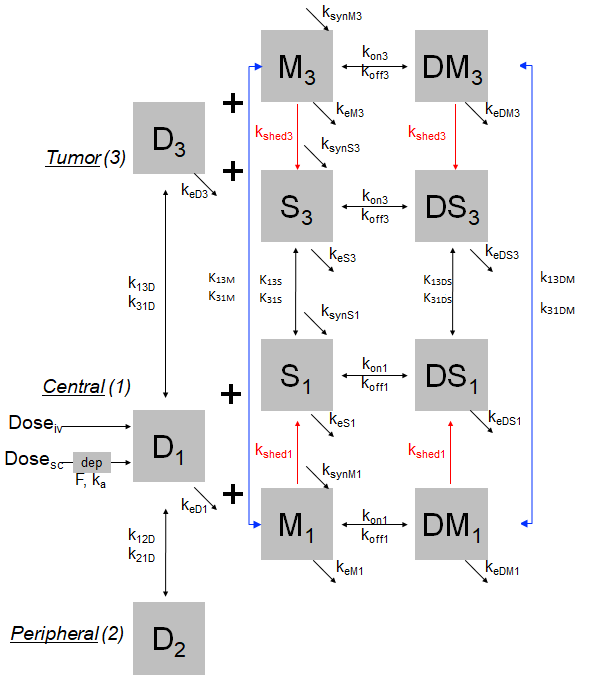
\includegraphics[scale=0.45]{figures/3compartment_shed_traffic.png}
\caption{Model.  THIS FIGURE NEEDS TO BE REDRAWN 
\label{fig:model}}.
\end{figure}

\begin{figure}[H]
\centering
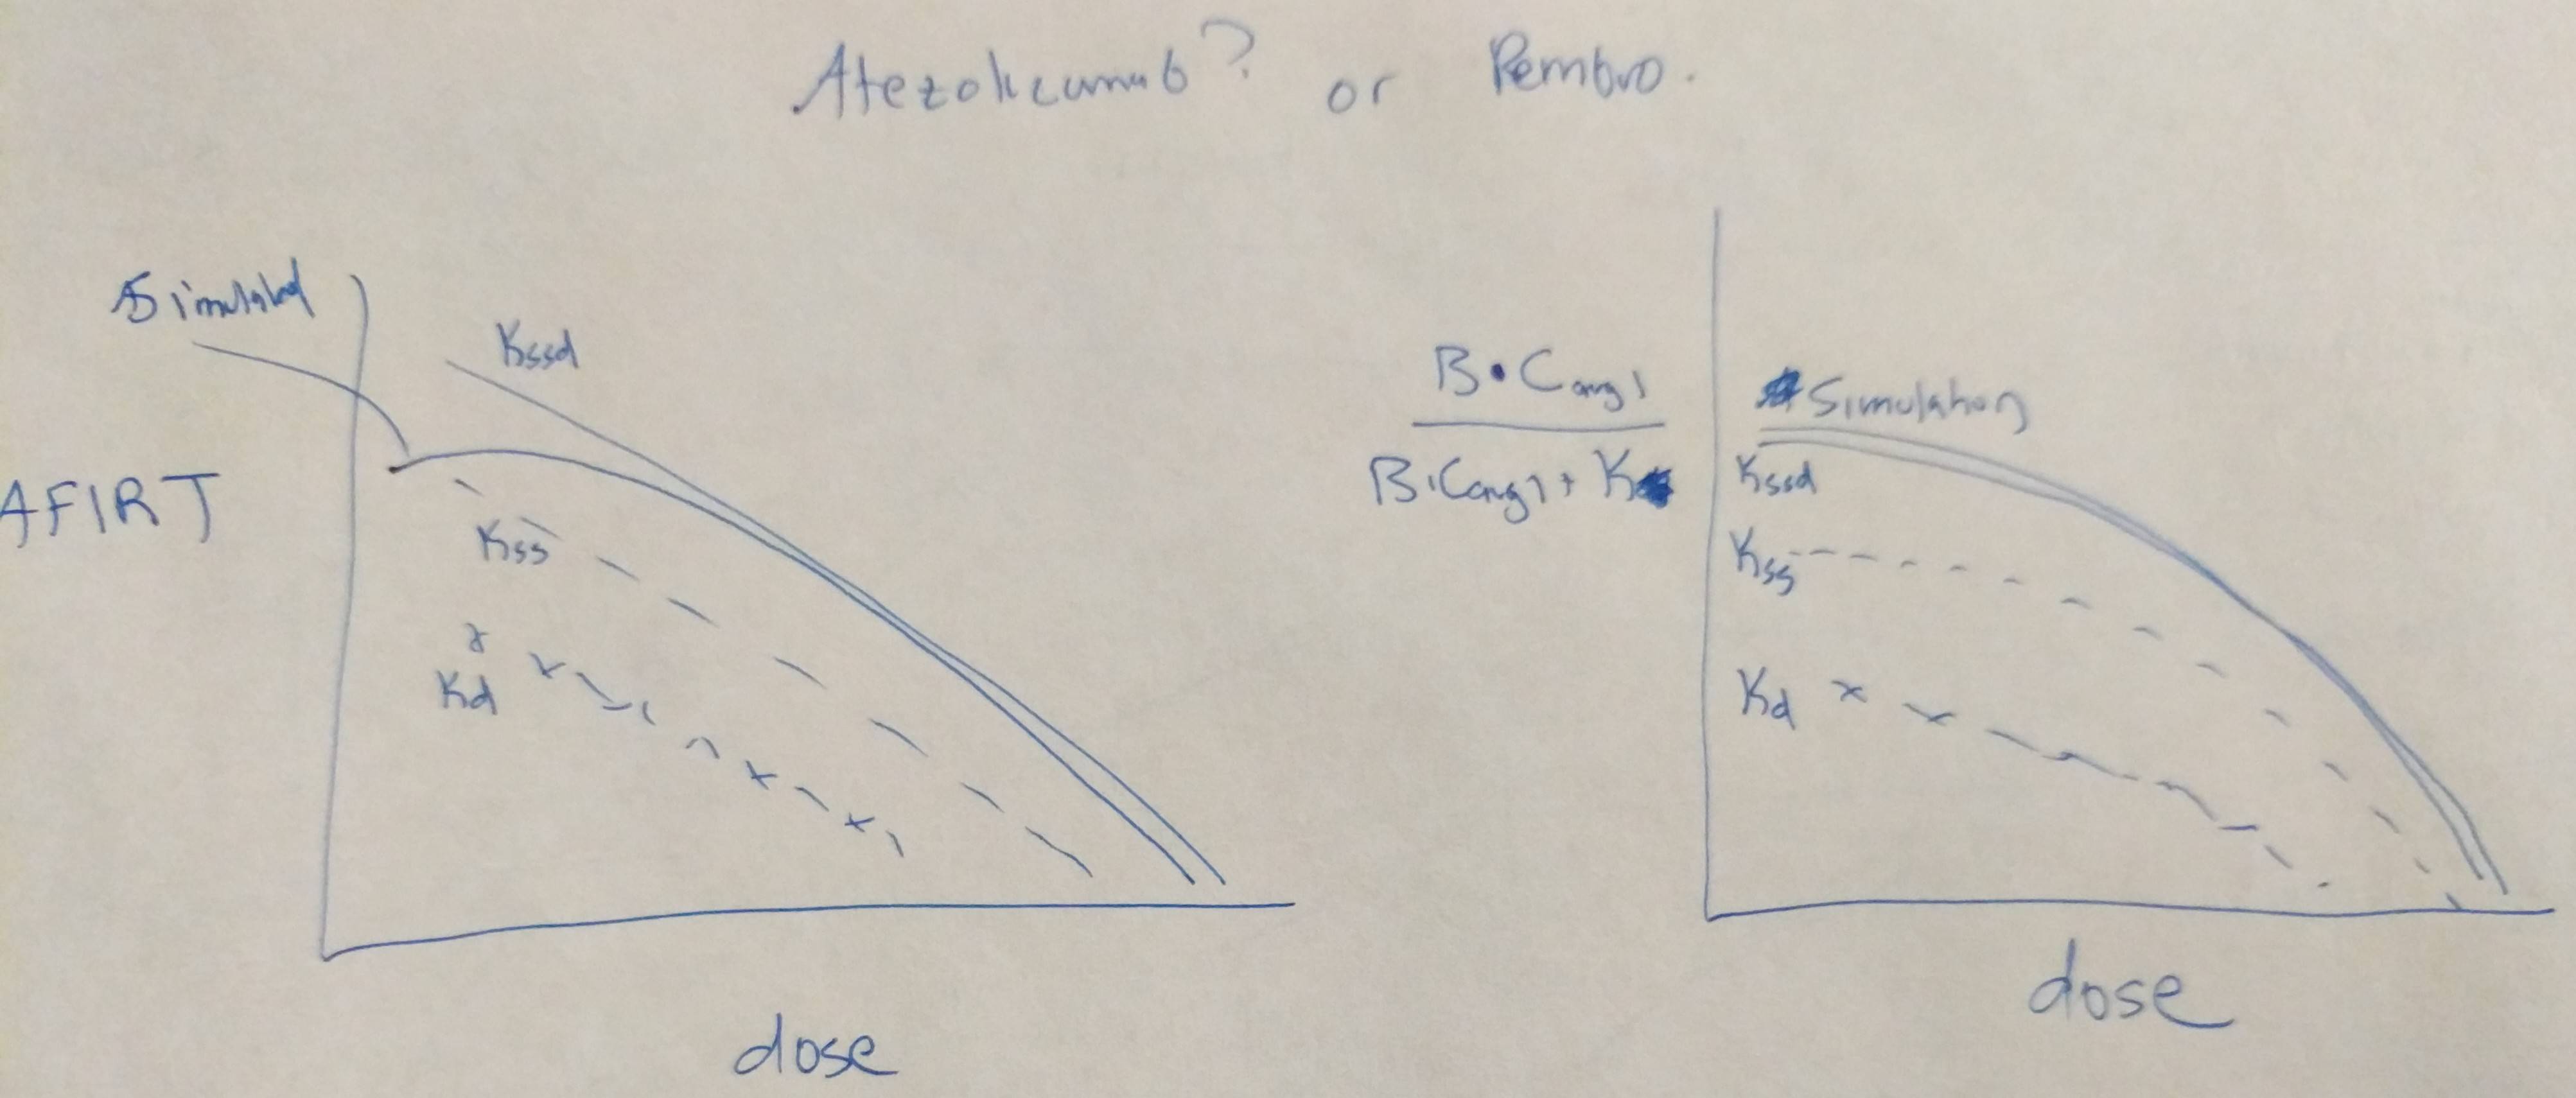
\includegraphics[width=\textwidth]{figures/Kssd_Kss_Kd.jpg}
\caption{Here we show Kd, Kss, Kssd and that Kssd is superior for describing the data.  Might want to show for all four drugs and that Kssd will be superior for atezo and pembro, though maybe all will be terrible for herceptin
\label{fig:Kssd}}.
\end{figure}

\begin{figure}[H]
\centering
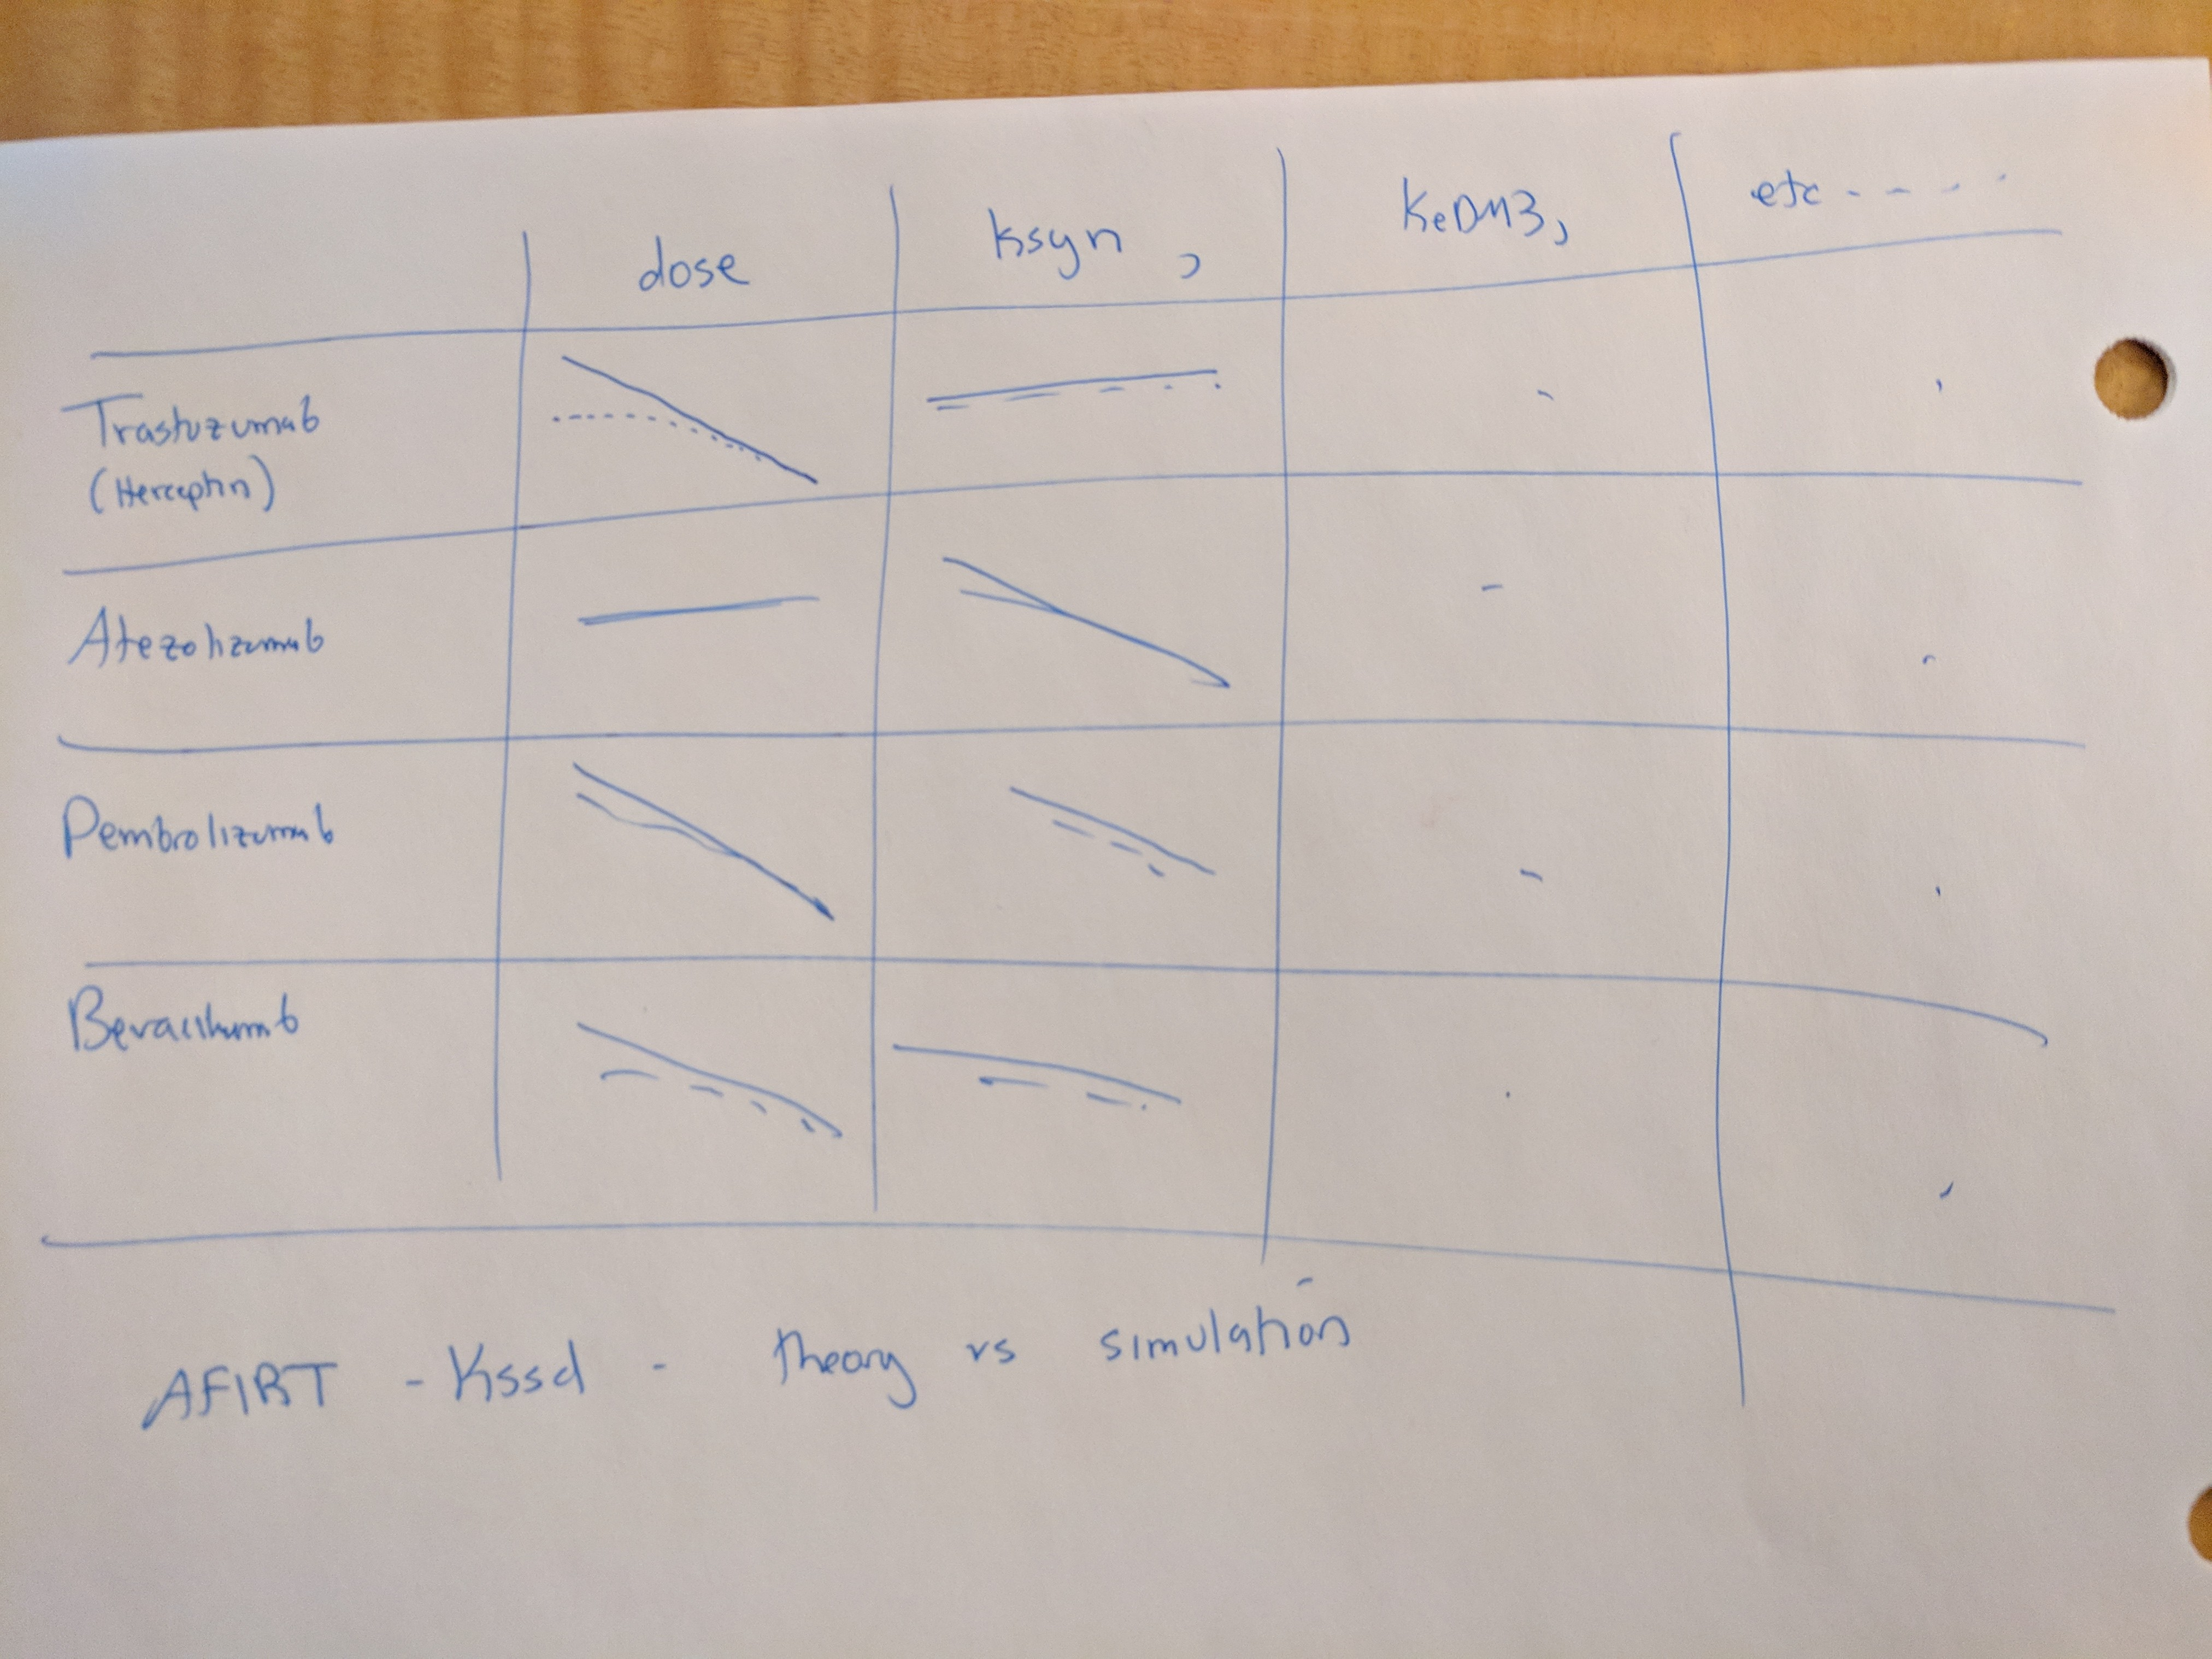
\includegraphics[width=\textwidth]{figures/SensitivityAnalysis.jpg}
\caption{Sensitivity analysis that Sameed is currently working on (building off Hongshan's initial code).  This will show the accuracy of the AFIRT (or lack there of) over a wide range of scenarios)
\label{fig:sensitivity}}.
\end{figure}

\begin{figure}[H]
\centering
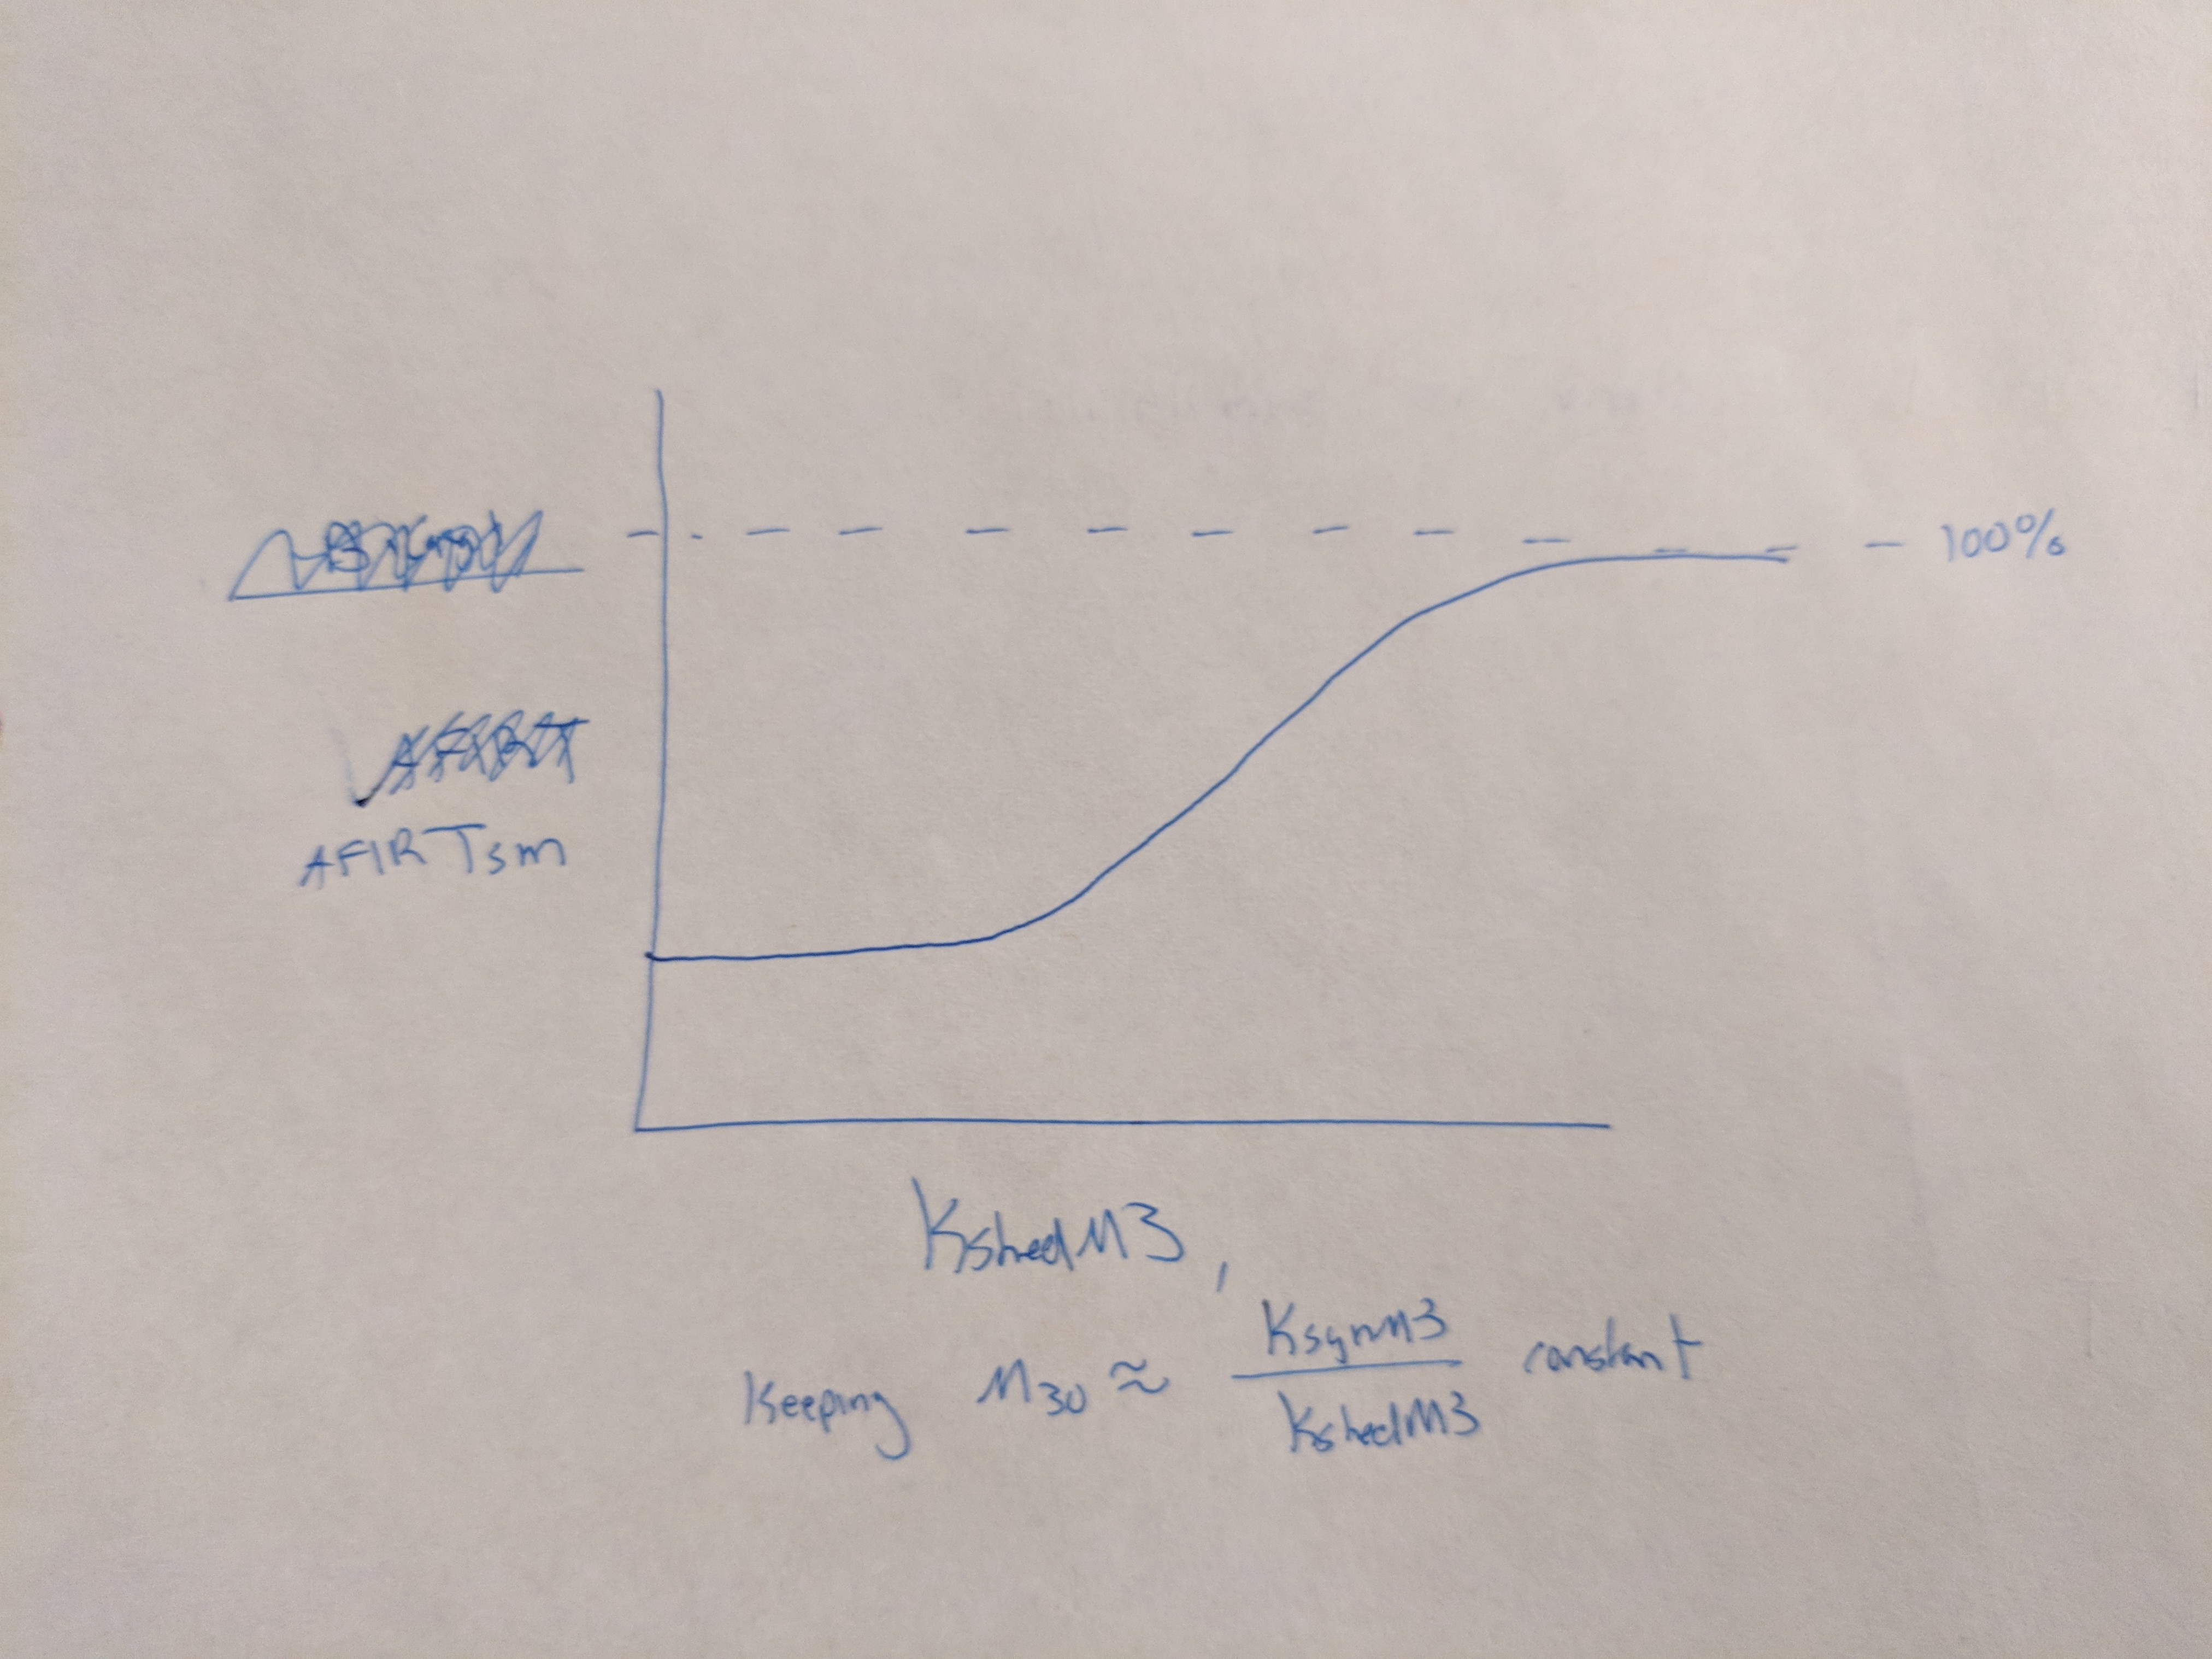
\includegraphics[width=\textwidth]{figures/FastShedding.jpg}
\caption{This will show that if the shedding is super fast, inhibiting the target is impossible.  This can also I think readily be seen from the Kssd equation. 
\label{fig:shedding}}.
\end{figure}

\begin{figure}[H]
\centering
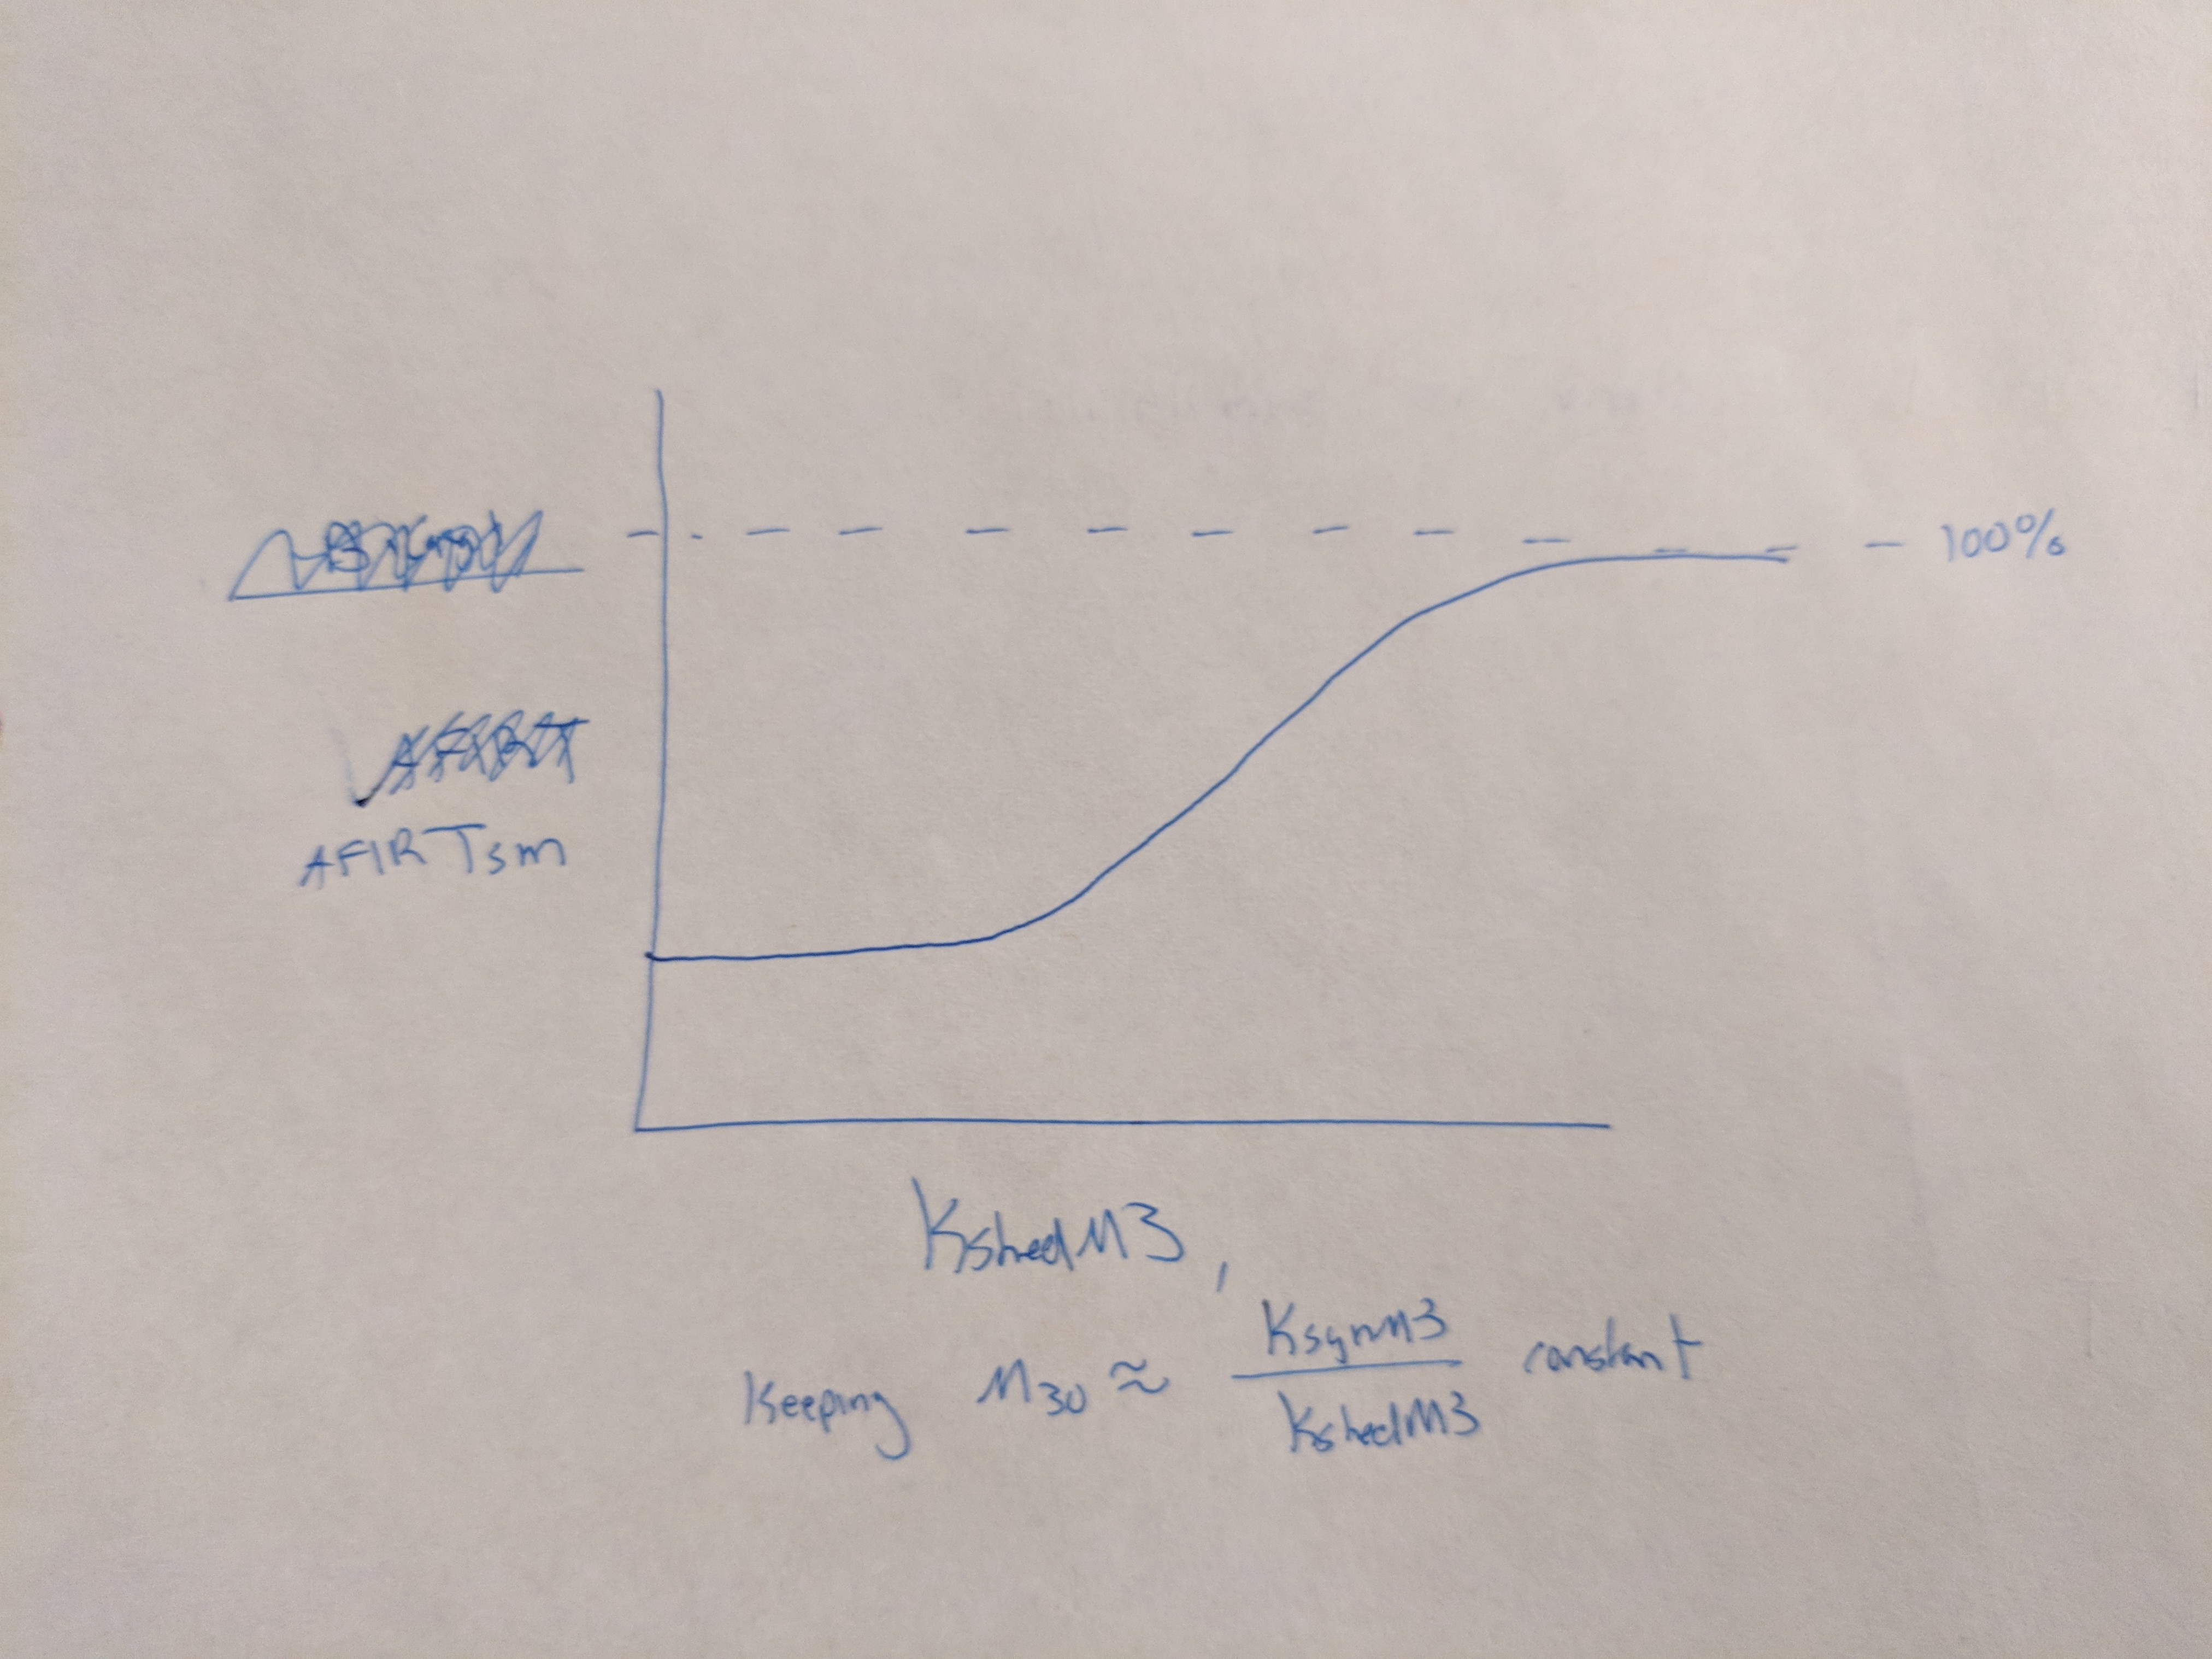
\includegraphics[width=\textwidth]{figures/FastShedding.jpg}
\caption{This will show that understanding the accumulation of the target in the tissue is critical.  But this is often not measured.  
\label{fig:accumulation}}.
\end{figure}

\end{document}
